% backmatter/anhang.tex

\chapter{Datensatz-Details}
\label{anh:datensatz}

\section{Modalitäten und Aktionsraum}
\label{anh:episodenstruktur}

Jede Episode im LeRobot-Format besteht aus zeitlich synchronisierten Kanälen
gemäß \cref{tab:anh-modalitaeten}. Zustands- und Aktionsvektor sind jeweils
28-dimensional und gleich gegliedert (\cref{tab:anh-aktionsraum}).

\begin{table}[htb]
  \centering
  \begin{tabularx}{\linewidth}{llX}
    \toprule
    Kanal & Dimension & Beschreibung \\
    \midrule
    \texttt{observation.images.cam\_left\_high}  & $3\times480\times640$ & RGB-Kopfkamera links \\
    \texttt{observation.images.cam\_right\_high} & $3\times480\times640$ & RGB-Kopfkamera rechts \\
    \texttt{observation.images.cam\_left\_wrist} & $3\times480\times640$ & RGB-Handgelenk links \\
    \texttt{observation.images.cam\_right\_wrist}& $3\times480\times640$ & RGB-Handgelenk rechts \\
    \texttt{observation.state}                   & 28 & Gelenkzustand (Arme und Hände) \\
    \texttt{action}                              & 28 & Soll-Aktion (Arme und Hände) \\
    \texttt{annotation.\dots}                    & -- & Aufgabenbeschreibung \\
    \bottomrule
  \end{tabularx}
  \caption{Modalitäten des Datensatzes G1\_Dex3\_BlockStacking.}
  \label{tab:anh-modalitaeten}
\end{table}

\begin{table}[htb]
  \centering
  \begin{tabular}{lll}
    \toprule
    Index & Gruppe & Repräsentation \\
    \midrule
    0--6   & linker Arm    & relative Gelenkänderungen \\
    7--13  & rechter Arm   & relative Gelenkänderungen \\
    14--20 & linke Hand    & absolute Gelenkwinkel \\
    21--27 & rechte Hand   & absolute Gelenkwinkel \\
    \bottomrule
  \end{tabular}
  \caption{Gliederung des 28-dimensionalen Aktions- und Zustandsvektors.}
  \label{tab:anh-aktionsraum}
\end{table}

\chapter{SLURM-Batch-Skript (Auszug)}
\label{anh:slurm}

\Cref{lst:anh-slurm} zeigt einen vereinfachten Auszug des für KISSKI verwendeten
Batch-Skripts. Charakteristisch sind die Einbindung des dauerhaften
Projektverzeichnisses nach \texttt{/data} und die Konfiguration ausschließlich
über Umgebungsvariablen. Das vollständige Skript liegt im Repository
(\doc{Training/kisski_submit.sh}), die Bedienung beschreibt
\doc{docs/training/kisski-hpc.md}.

\begin{listing}[htb]
\begin{minted}{bash}
#!/usr/bin/env bash
#SBATCH --job-name=groot-finetune
#SBATCH --partition=kisski            # A100 80 GB (alt.: kisski-h100)
#SBATCH -G A100:1                     # 4x A100 fuer den Multi-GPU-Lauf
#SBATCH -c 16
#SBATCH --mem=64G
#SBATCH --time=48:00:00
#SBATCH --output=logs/slurm-%j.out

module load apptainer

apptainer exec --nv \
  --bind /mnt/vast-kisski/projects/kisski-humrob/data:/data \
  --env HF_TOKEN="${HF_TOKEN}" \
  --env WANDB_API_KEY="${WANDB_API_KEY:-}" \
  --env GLOBAL_BATCH_SIZE="${GLOBAL_BATCH_SIZE:-8}" \
  --env MAX_STEPS="${MAX_STEPS:-44000}" \
  --env NUM_GPUS="${NUM_GPUS:-1}" \
  "${SIF_IMAGE}" \
  bash /scripts/entrypoint.sh
\end{minted}
\caption{Vereinfachter Auszug aus \texttt{kisski\_submit.sh}.}
\label{lst:anh-slurm}
\end{listing}

\chapter{Software, Versionen und Reproduzierbarkeit}
\label{anh:software}

\begin{table}[htb]
  \centering
  \begin{tabular}{ll}
    \toprule
    Komponente       & Version \\
    \midrule
    Python (Training)         & 3.10 \\
    CUDA                      & 12.8 \\
    Paketmanager              & \texttt{uv} \\
    DeepSpeed                 & 0.17.6 \\
    Weights \& Biases         & 0.23.0 \\
    Simulation bis Juli 2026  & Isaac~Lab~2.3.2 mit Isaac~Sim~5.1 (Python~3.11) \\
    Simulation ab Aug.\ 2026  & Isaac~Lab~3.0.0-beta2 mit Isaac~Sim~6.0 (Python~3.12) \\
    GR00T                     & Fork \texttt{lucam06/Isaac-GR00T}, Commit \texttt{26ad1f7} \\
    \bottomrule
  \end{tabular}
  \caption{Software-Versionen der Trainings- und Simulationsumgebung. Die
    Umstellung auf Isaac~Sim~6.0 war durch die Blackwell-GPUs des
    Institutsservers erzwungen (\cref{sec:hindernisse}).}
  \label{tab:anh-software}
\end{table}

Code, Dokumentation und Diagnoseprotokoll liegen im Repository
\url{https://github.com/Docboter/projektarbeit_humanoider_roboter}
(Branch \texttt{training-luca-IKR-IS6.0}, Stand dieser Arbeit: Commit
\texttt{853fd71}). Die Trainingsläufe sind im \ac{wandb}-Projekt
\texttt{gr00t-g1-dex3} protokolliert, die für die Simulation verwendeten
Checkpoints liegen auf Hugging Face (\texttt{luca-mue/groot-g1dex3-checkpoint}
und Varianten). Der Einstieg für eine Reproduktion ist \doc{docs/quickstart.md}.

\chapter{Trainingsdynamik: Lernrate und Gradientennorm}
\label{anh:trainingsdynamik}

Ergänzend zum Loss-Verlauf (\cref{fig:loss-curve}) zeigen die beiden folgenden
Abbildungen Lernrate und Gradientennorm der drei Läufe aus \ac{wandb}. Die
Lernrate ist durch die Konfiguration vorgegeben, die Gradientennorm ist ein
gemessenes Diagnosesignal.

\begin{figure}[htb]
  \centering
  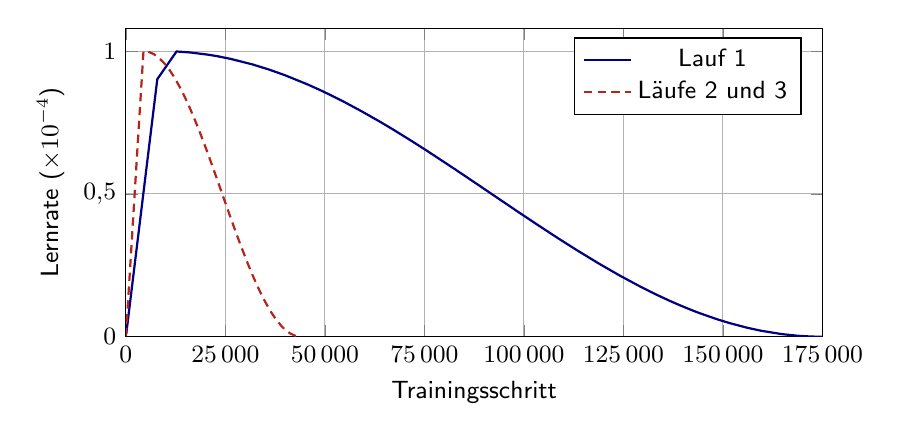
\begin{tikzpicture}
    \begin{axis}[
      width  = 0.86\textwidth,
      height = 5.5cm,
      xlabel = {Trainingsschritt},
      ylabel = {Lernrate ($\times 10^{-4}$)},
      grid   = both,
      grid style = {line width=0.2pt, draw=gray!30},
      major grid style = {line width=0.4pt, draw=gray!60},
      xmin = 0, xmax = 175000, ymin = 0, ymax = 1.08,
      xtick distance = 25000,
      scaled x ticks = false,
      x tick label style = {/pgf/number format/.cd, set thousands separator={\,}, fixed},
      legend pos = north east,
      legend style = {font=\small\sffamily},
      tick label style = {font=\small\sffamily},
      label style = {font=\small\sffamily},
      y tick label style = {/pgf/number format/.cd, use comma},
    ]
      \addplot[NavyBlue, thick] coordinates { 
        (80,0.0090) (4720,0.5393) (7890,0.9016) (12720,0.9986) (16110,0.9952) (20710,0.9873)
        (23190,0.9815) (26110,0.9733) (31710,0.9537) (35770,0.9362) (39820,0.9163) (45630,0.8834)
        (48520,0.8653) (51280,0.8470) (54710,0.8230) (59220,0.7893) (64220,0.7496) (67320,0.7238)
        (71520,0.6876) (75720,0.6503) (82660,0.5866) (89100,0.5262) (93720,0.4826) (98050,0.4418)
        (102850,0.3971) (108590,0.3447) (113300,0.3031) (118820,0.2563) (124180,0.2134)
        (129200,0.1759) (133260,0.1476) (136700,0.1253) (139330,0.1094) (142130,0.0934)
        (144030,0.0832) (148350,0.0621) (151420,0.0488) (156110,0.0315) (159570,0.0211)
        (164750,0.0094) (168820,0.0034) (172270,0.0007) (174960,0.0000)
       };
      \addlegendentry{Lauf~1}
      \addplot[BrickRed, thick, densely dashed] coordinates { 
        (10,0.0020) (1030,0.2339) (2140,0.4861) (2930,0.6657) (4420,1.0000) (5600,0.9977)
        (6850,0.9906) (7900,0.9809) (9390,0.9613) (10160,0.9487) (11070,0.9316) (12160,0.9082)
        (13660,0.8711) (14340,0.8525) (15300,0.8245) (15980,0.8035) (17550,0.7517) (18780,0.7085)
        (19920,0.6666) (20530,0.6436) (21730,0.5974) (22260,0.5767) (22830,0.5543) (23550,0.5258)
        (24850,0.4743) (25580,0.4454) (26500,0.4093) (27580,0.3676) (28830,0.3205) (30670,0.2545)
        (31710,0.2195) (32760,0.1860) (33890,0.1524) (34630,0.1319) (35820,0.1017) (36720,0.0811)
        (37760,0.0600) (39130,0.0369) (39820,0.0273) (41200,0.0123) (42530,0.0034) (43190,0.0010)
        (43970,0.0000)
       };
      \addlegendentry{Läufe~2 und 3}
    \end{axis}
  \end{tikzpicture}
  \caption{Lernrate der Läufe. Lineares Warmup auf $1{,}0\times10^{-4}$
    (Lauf~1: 5\,\% der Schritte, Läufe~2 und~3: 10\,\%), danach Cosine-Abfall
    auf null. Die Kurven von Lauf~2 und Lauf~3 sind identisch.}
  \label{fig:anh-lr}
\end{figure}

\begin{figure}[htb]
  \centering
  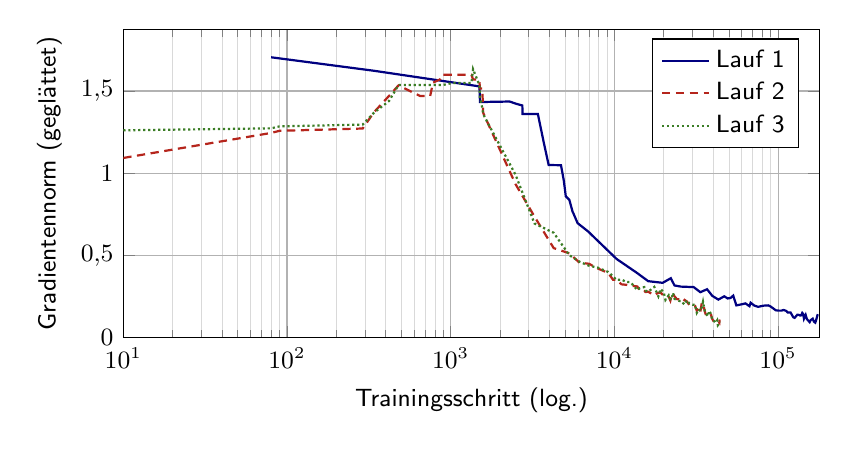
\begin{tikzpicture}
    \begin{semilogxaxis}[
      width  = 0.86\textwidth,
      height = 5.5cm,
      xlabel = {Trainingsschritt (log.)},
      ylabel = {Gradientennorm (geglättet)},
      grid   = both,
      grid style = {line width=0.2pt, draw=gray!30},
      major grid style = {line width=0.4pt, draw=gray!60},
      xmin = 10, xmax = 180000, ymin = 0,
      legend pos = north east,
      legend style = {font=\small\sffamily},
      tick label style = {font=\small\sffamily},
      label style = {font=\small\sffamily},
      y tick label style = {/pgf/number format/.cd, use comma},
    ]
      \addplot[NavyBlue, thick] coordinates {
        (80,1.705) (340,1.623) (1500,1.528) (1510,1.433) (2290,1.436) (2340,1.433) (2520,1.422)
        (2740,1.412) (2750,1.360) (3410,1.360) (3710,1.184) (3970,1.050) (4720,1.049) (4910,0.956)
        (5050,0.860) (5310,0.838) (5560,0.765) (5600,0.760) (5960,0.697) (6410,0.672) (6900,0.647)
        (10320,0.479) (13710,0.395) (16100,0.344) (19740,0.334) (22120,0.362) (23300,0.318)
        (25480,0.311) (30520,0.308) (33520,0.277) (36850,0.295) (39640,0.255) (43150,0.232)
        (46920,0.252) (49210,0.239) (51230,0.242) (53230,0.256) (55620,0.197) (59780,0.203)
        (63160,0.209) (66910,0.192) (68010,0.213) (71580,0.196) (75660,0.188) (81130,0.195)
        (86890,0.197) (89410,0.192) (93070,0.180) (96820,0.167) (100770,0.165) (104900,0.165)
        (108070,0.169) (112320,0.163) (114630,0.153) (119190,0.154) (123820,0.125) (126220,0.121)
        (131120,0.140) (134120,0.139) (136670,0.135) (138250,0.136) (140590,0.151) (142480,0.144)
        (143990,0.116) (147440,0.139) (150040,0.114) (151720,0.108) (155990,0.095) (158140,0.107)
        (162830,0.116) (165670,0.098) (168750,0.092) (170490,0.104) (174410,0.140) (174960,0.143)
      };
      \addlegendentry{Lauf~1}
      \addplot[BrickRed, thick, densely dashed] coordinates {
        (10,1.093) (80,1.245) (90,1.258) (290,1.272) (340,1.371) (420,1.470) (480,1.534)
        (650,1.470) (750,1.470) (780,1.551) (860,1.570) (890,1.599) (1030,1.599) (1050,1.599)
        (1340,1.599) (1370,1.570) (1480,1.570) (1500,1.551) (1510,1.515) (1560,1.515) (1580,1.367)
        (2490,0.934) (3250,0.737) (4260,0.545) (5310,0.513) (6130,0.456) (6990,0.450) (7890,0.422)
        (9170,0.394) (9810,0.353) (10320,0.353) (11040,0.325) (11820,0.322) (12550,0.317)
        (13810,0.312) (14330,0.285) (15240,0.285) (15470,0.278) (16100,0.280) (17540,0.258)
        (18570,0.274) (19190,0.274) (20030,0.255) (20520,0.250) (21480,0.249) (21990,0.226)
        (22280,0.249) (22810,0.270) (23300,0.252) (24100,0.235) (24940,0.234) (25480,0.228)
        (26370,0.219) (26840,0.230) (27730,0.221) (28730,0.199) (29980,0.195) (31130,0.194)
        (31890,0.164) (32730,0.181) (33520,0.157) (34200,0.211) (34800,0.211) (35790,0.156)
        (36450,0.133) (37120,0.133) (38050,0.143) (38990,0.139) (39550,0.117) (40210,0.103)
        (41510,0.105) (42470,0.109) (42890,0.102) (43790,0.091) (43970,0.111)
      };
      \addlegendentry{Lauf~2}
      \addplot[OliveGreen, thick, densely dotted] coordinates {
        (10,1.261) (80,1.273) (90,1.285) (290,1.296) (340,1.368) (420,1.439) (480,1.536)
        (650,1.536) (750,1.536) (780,1.536) (860,1.536) (890,1.536) (1030,1.549) (1050,1.549)
        (1340,1.549) (1370,1.633) (1480,1.549) (1500,1.536) (1510,1.463) (1560,1.396) (1580,1.359)
        (2490,0.991) (3250,0.695) (4260,0.638) (5310,0.502) (6130,0.462) (6990,0.438) (7890,0.427)
        (9170,0.400) (9810,0.374) (10320,0.351) (11040,0.354) (11820,0.339) (12550,0.338)
        (13810,0.290) (14330,0.302) (15240,0.308) (15470,0.287) (16100,0.280) (17540,0.309)
        (18570,0.252) (19190,0.297) (20030,0.276) (20520,0.230) (21480,0.258) (21990,0.235)
        (22280,0.231) (22810,0.273) (23300,0.237) (24100,0.230) (24940,0.224) (25480,0.224)
        (26370,0.209) (26840,0.202) (27730,0.228) (28730,0.208) (29980,0.201) (31130,0.201)
        (31890,0.152) (32730,0.173) (33520,0.162) (34200,0.185) (34800,0.219) (35790,0.154)
        (36450,0.145) (37120,0.130) (38050,0.164) (38990,0.143) (39550,0.110) (40210,0.108)
        (41510,0.090) (42470,0.106) (42890,0.076) (43790,0.086) (43970,0.098)
      };
      \addlegendentry{Lauf~3}
    \end{semilogxaxis}
  \end{tikzpicture}
  \caption{Gradientennorm der drei Läufe (gleitender Median über 15~Werte,
    logarithmische Abszisse). Alle Läufe erreichen in der Warmup-Phase ein
    Maximum von etwa 1,6 bis 1,7 und fallen danach auf 0,1 bis 0,15. Spitzen
    oder Divergenzen treten nicht auf, auch nicht bei mittrainiertem
    Bild-Encoder.}
  \label{fig:anh-gradnorm}
\end{figure}

\chapter{Simulations-Diagnostik}
\label{anh:sim-diagnostik}

\section{Open-Loop-Aktionsvergleich}
\label{anh:openloop}

\Cref{fig:anh-openloop} zeigt den Open-Loop-Test aus \cref{sec:diagnose} im
Detail. Für jede der 28~Aktionsdimensionen wird die vom Modell auf realen
Bildern vorhergesagte Aktion der aufgezeichneten gegenübergestellt. Die
Armdimensionen (0--13) folgen dem Referenzverlauf gut, die Fingerdimensionen
(14--27) sind deutlich verrauscht. Die gezeigte Episode~0 war im ersten Lauf
Teil der Trainingsdaten.

\begin{figure}[p]
  \centering
  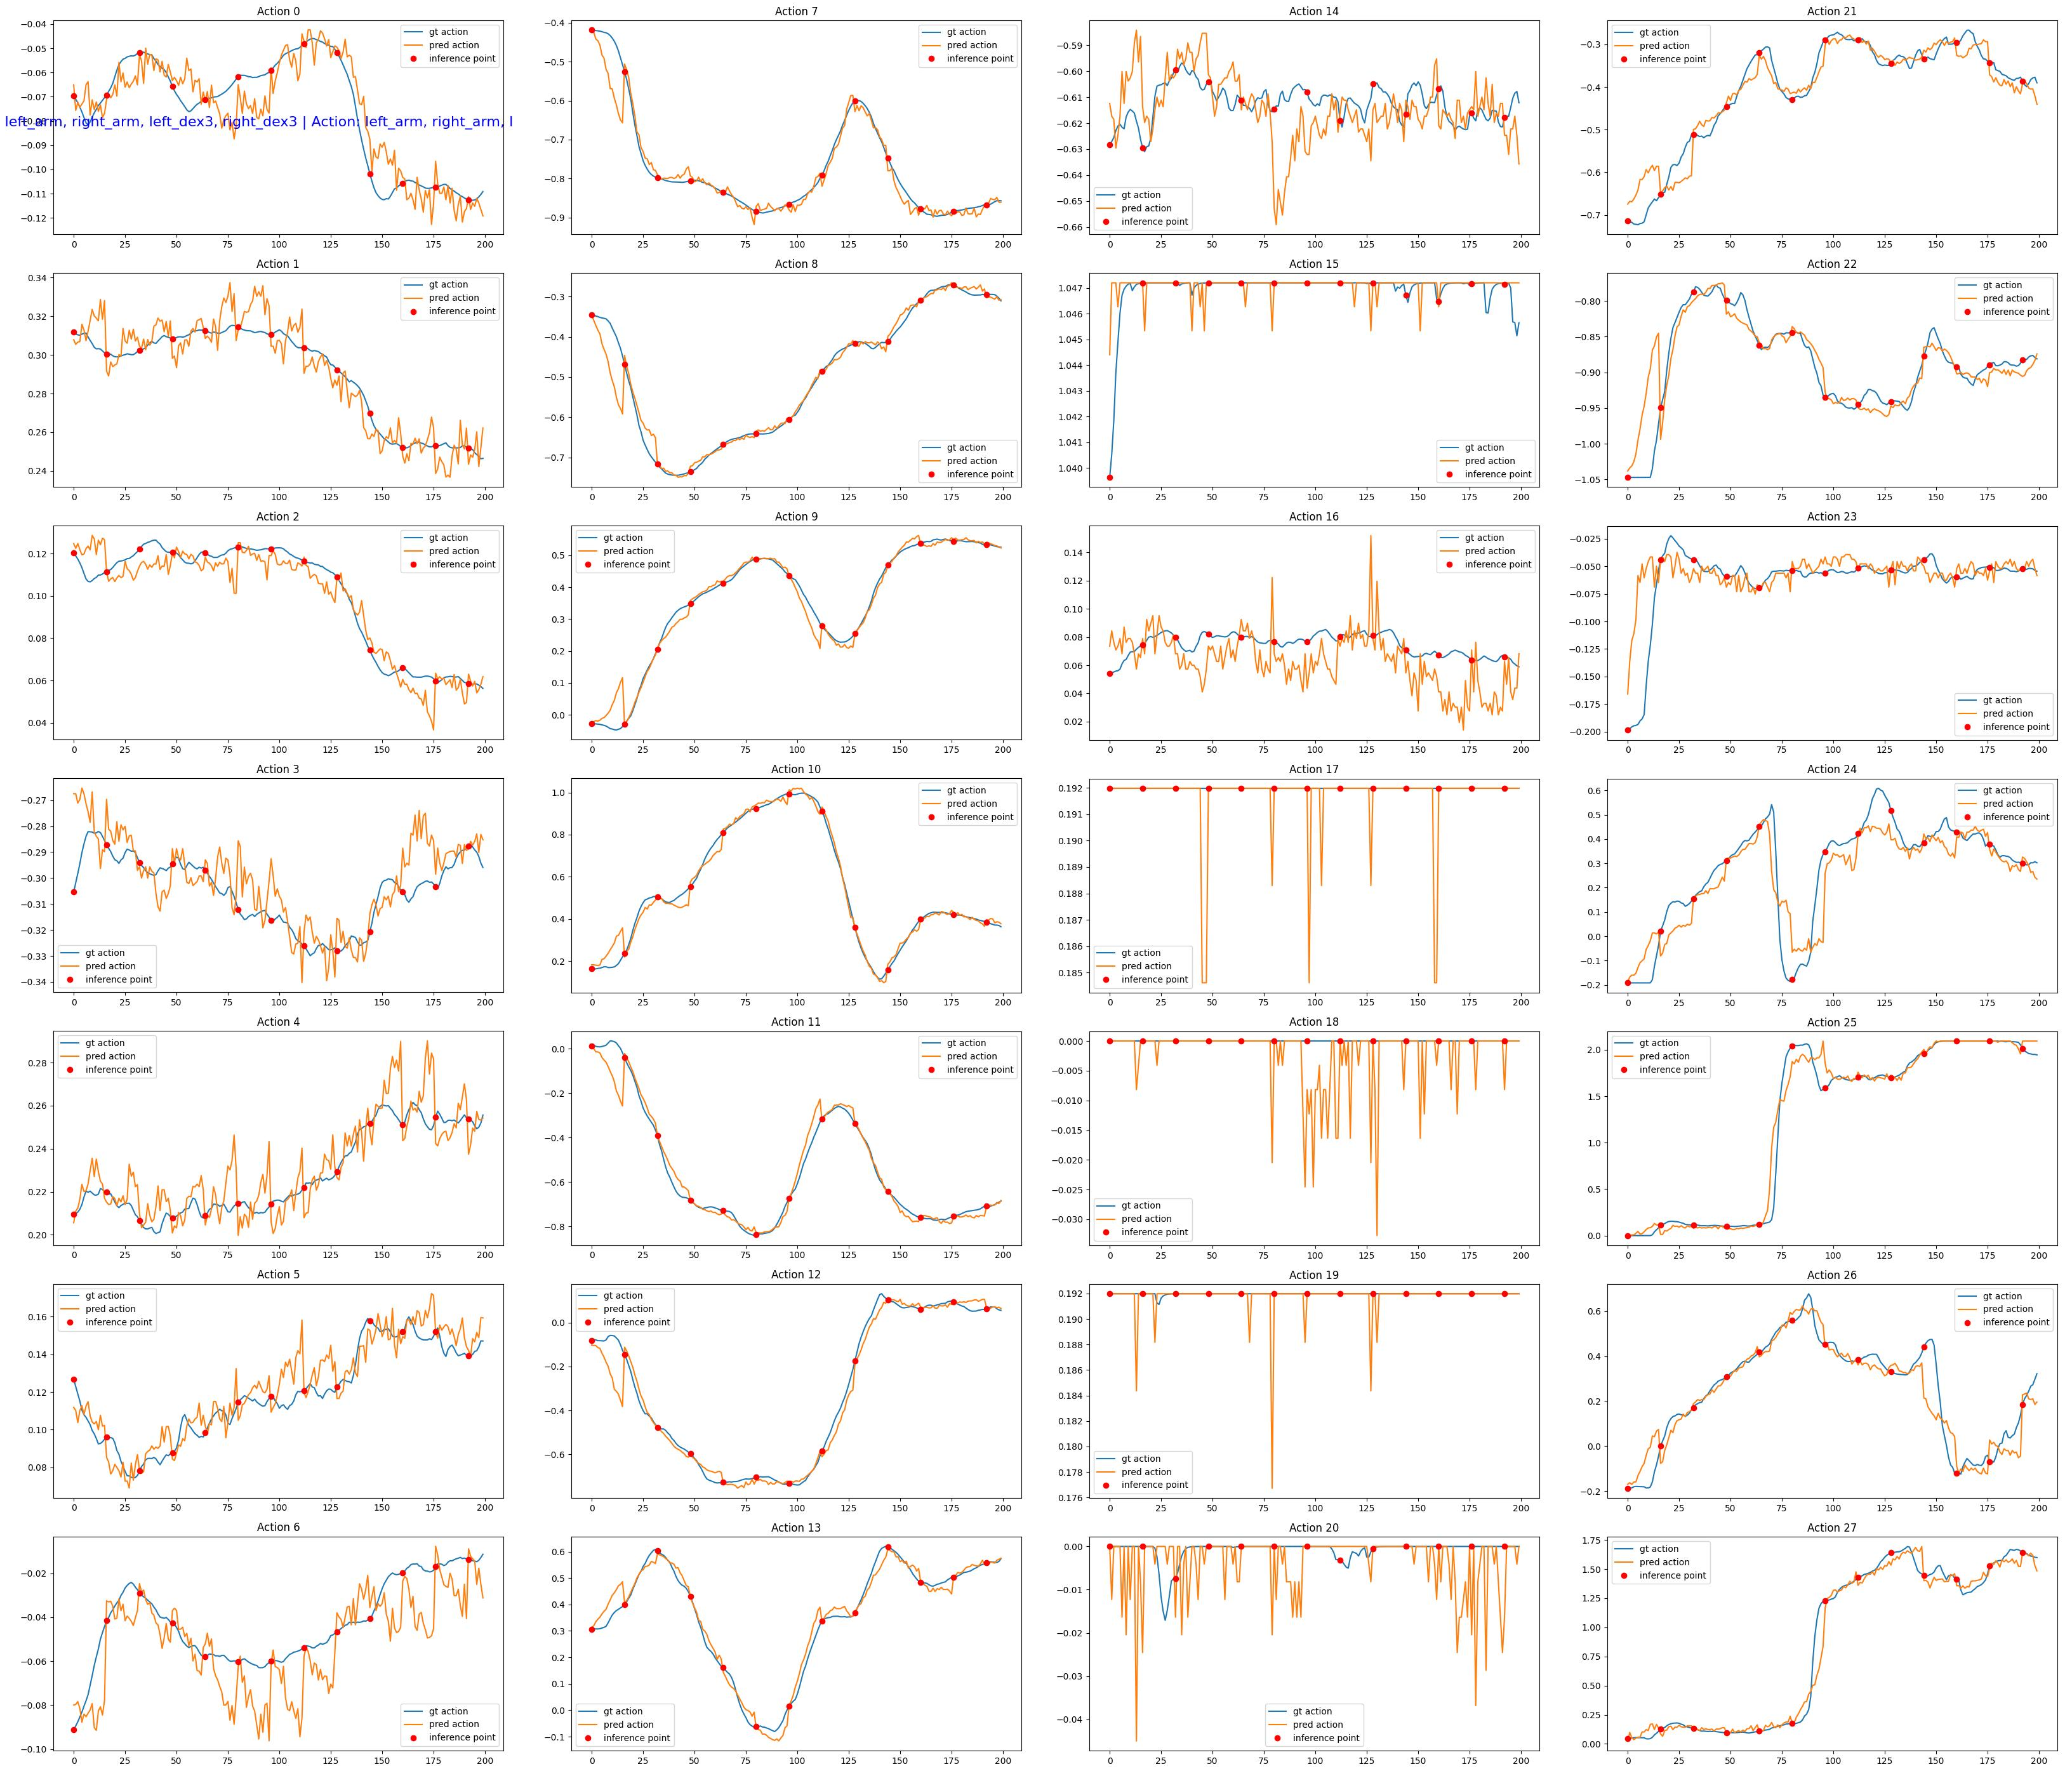
\includegraphics[width=\linewidth]{figures/sim/openloop_montage.png}
  \caption{Open-Loop-Aktionsvergleich für den letzten Checkpoint des ersten
    Laufs (Episode~0). Die 28~Aktionsdimensionen sind spaltenweise angeordnet
    (Spalte~1: linker Arm~0--6, Spalte~2: rechter Arm~7--13, Spalte~3: linke
    Hand~14--20, Spalte~4: rechte Hand~21--27). Pro Dimension: aufgezeichnete
    Aktion (blau), Vorhersage (orange) und Referenzpunkte (rot).}
  \label{fig:anh-openloop}
\end{figure}

\section{Parameter der Simulationsszene}
\label{anh:szenenparameter}

\Cref{tab:anh-szene} fasst die Parameter der Simulationsszene vor und nach den
Korrekturen aus \cref{sec:geometrie} zusammen.

\begin{table}[htb]
  \centering
  \begin{tabularx}{\linewidth}{lllX}
    \toprule
    Parameter & Alt & Neu & Bedeutung \\
    \midrule
    Beckenhöhe          & 0,85~m   & 0,764~m  & Höhe der Roboterbasis über dem Boden \\
    Basis $x$           & 0        & $-$0,057~m & Längsversatz der Roboterbasis \\
    Würfel-Ruhehöhe     & 0,915~m  & 0,895~m  & Tisch 0,87~m plus halbe Kantenlänge \\
    Vorzeichenumkehr    & 4 Gelenke & keine   & Fingergrundgelenke (\cref{sec:geometrie}) \\
    Sichtfeld Kopfkameras & 47,2°  & 75,0°    & zuvor durch einen Fehler nie angewendet \\
    Abstand Kopfkameras & --       & $\pm$0,025~m & aus der Pixel-Disparität des realen
      Kamerapaars bestimmt, parallel ausgerichtet \\
    Würfeldrehung       & stets 0° & offen    & real nahezu gleichverteilt über 0--45° \\
    \bottomrule
  \end{tabularx}
  \caption{Parameter der Simulationsszene vor und nach den Korrekturen
    (\doc{docs/ergebnisse/diagnose-chronik.md}).}
  \label{tab:anh-szene}
\end{table}

\section{Kamerakalibrierung über Überlagerungen}
\label{anh:overlay}

Die Kamerakalibrierung aus \cref{sec:kalibrierung} erfolgte mangels
Kalibrierdaten iterativ: Das erste reale Bild einer Episode und das erste
simulierte Bild wurden halbtransparent überlagert und die Kamerapose in der
Simulation so lange angepasst, bis Tischkanten, Würfel und Hände zur Deckung
kamen (\cref{fig:anh-overlay}).

\begin{figure}[htb]
  \centering
  \begin{subfigure}{\linewidth}
    \centering
    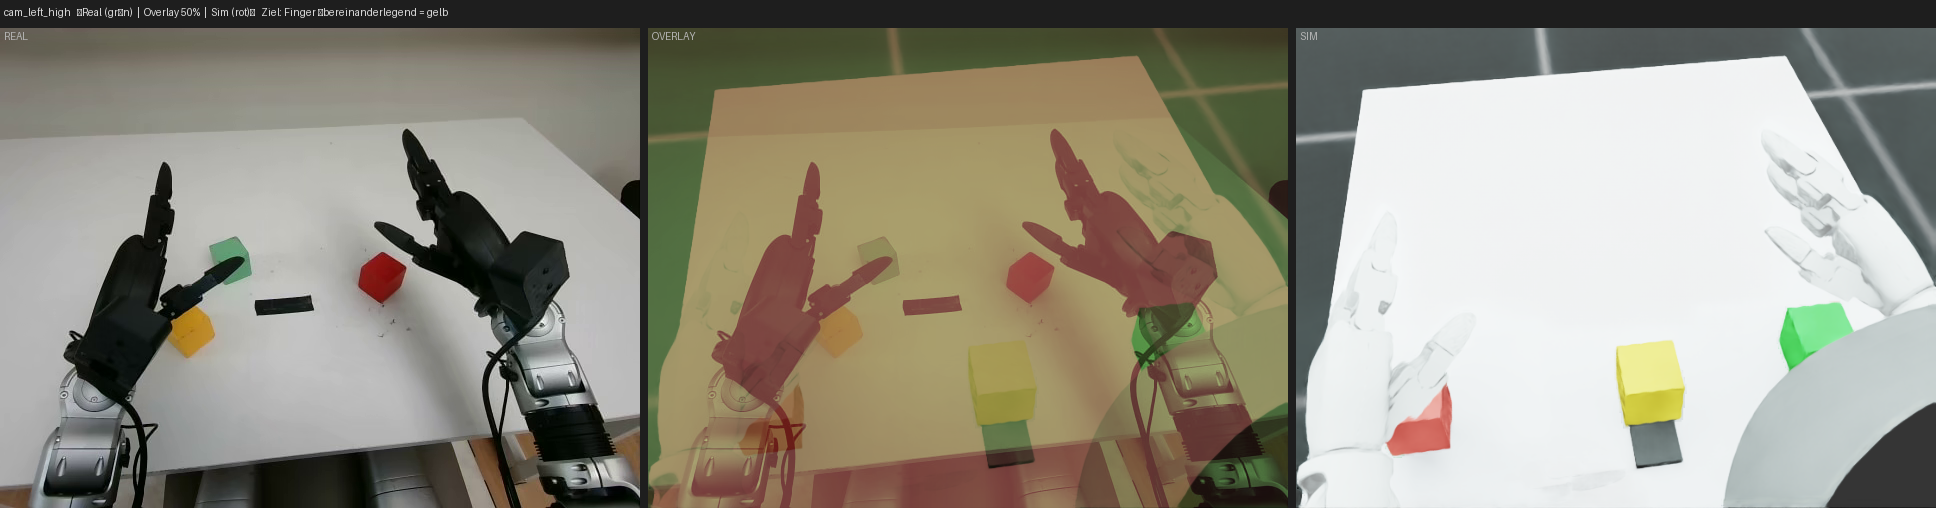
\includegraphics[width=\linewidth]{figures/sim/panel_cam_left_high.png}
    \caption{Kopfkamera links}
    \label{fig:anh-overlay-high}
  \end{subfigure}\\[0.6em]
  \begin{subfigure}{\linewidth}
    \centering
    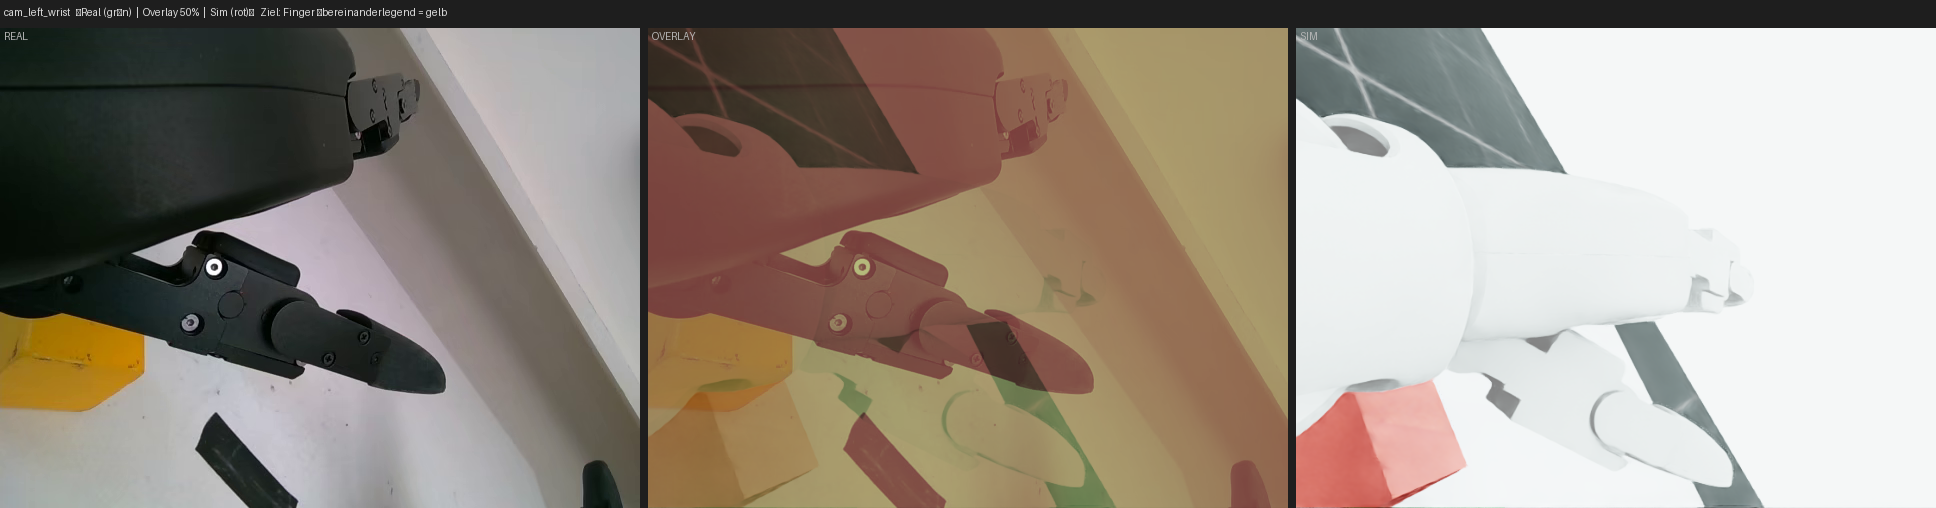
\includegraphics[width=\linewidth]{figures/sim/panel_cam_left_wrist.png}
    \caption{Handgelenkkamera links}
    \label{fig:anh-overlay-wrist}
  \end{subfigure}
  \caption{Kamerakalibrierung über Überlagerungen (Stand Juni~2026), je Panel
    von links nach rechts: reales Bild, Überlagerung, simuliertes Bild. Die
    linke Handgelenkkamera (b) wies im Juni mit einer Cosinus-Distanz von
    0,427 den größten Domain-Gap auf (\cref{tab:domain-gap}).}
  \label{fig:anh-overlay}
\end{figure}
